\documentclass[journal=jacsat,manuscript=article]{achemso}
% \linespread{1.5}
% \usepackage{amssymb,amsmath,graphics,epsfig}
\usepackage{amsmath}
\usepackage[font=small,labelfont=bf]{caption}
\setkeys{acs}{super = true}
\setcitestyle{super,open={},close={}}
\def\citenumfont{}

% \usepackage[version=3]{mhchem} 
\usepackage{color}
\newcommand{\eqnref}[1]{Eqn.~\plainref{#1}}
\newcommand{\figref}[1]{Fig.~\plainref{#1}}
\newcommand{\tabref}[1]{Table~\plainref{#1}}

\title{Making Soup: Preparing and Validating Molecular Simulations of the Bacterial Cytoplasm}

\author{Zahedeh Bashardanesh}
\affiliation{Science for Life Laboratory, Department of Cell and Molecular Biology. Uppsala University, SE-751 05 Uppsala, Sweden}

\author{Leandro Oliveira Bortot}
\affiliation{Laboratory of Biological Physics, School of Pharmaceutical Sciences of Ribeir{\~a}o Preto, University of S{\~a}o Paulo, Ribeir{\~a}o Preto, Brazil}

\author{David van der Spoel}
\affiliation{Science for Life Laboratory, Department of Cell and Molecular Biology. Uppsala University, SE-751 05 Uppsala, Sweden}
\email{david.vanderspoel@icm.uu.se}


\begin{document}

\maketitle

\begin{abstract}
%For Nature, the abstract is really an introductory paragraph set
%in bold type.  This paragraph must be ``fully referenced'' and
%less than 180 words for Letters.  This is the thing that is
%supposed to be aimed at people from other disciplines and is
%arguably the most important part to getting your paper past the
%editors.  End this paragraph with a sentence like ``Here we
%show...'' or something similar.

 
\end{abstract}
\section*{Introduction}

Biomolecules move and function in an environment densely packed with high concentrations of macromolecules. The presence of macromolecules leads to steric effect due to excluded volume effect and intermolecular attrative/repulsive forces due to distributed charges on the surface of macromolecules.

Structure and dynamics of biomolecules are well characterized {\em in vitro}, however how these features differ {\em in vivo} remains unclear. 
Investigating biomolecular properties {\em in vivo} is possible through development in the fields of nuclear magnetic resonance~\cite{reckel2007,pielak2008}, or fluoroscence spectroscopies~\cite{ignatova2004,xie2008,English2011}.
An alternative is to use computational models and simulations techniques. Biomolecular simulations are often carried out under dilute conditions or simple models of macromolecular crowdings~\cite{Spiga2014a,Harada2012a,Nawrocki2017a}. However, more attemps in modeling bacterial cytoplasm have been made recently~\cite{Mcguffee2010,Yu2016a}. 

Here we report on a model of {\em Escherichia coli} cytoplasm at atomistic level. The challenges in modeling and simulation with Molecular Dynamics are pointed and discussed and solutions are provided. 

This work is the first model of {\em E. coli} at atomistic resolution that spans cellular dynamics on a microsecond scale.




\section*{Materials and Methods}


\subsection*{Initial structures}
The proteins and tRNA were downloaded from Protein Data Bank (PDB). We looked for the proteins structures that were either from or expressed in {\em E-coli}. In case of 1U22 (MetE) and 2EIP (Ppa) we used a loop-closure modelng tool based on Random Coordinate Descent (RCD) method~\cite{Chys2013} to correct the information for missing residues. The four metabolites were parametrized using GAFF and Antechamber. 

\subsection*{Molecular Dynamics Simulation}

 
{\bf General Simulation Setup: }The proteins were simulated at 30\% biomolecular mass fraction in  a physiological salt concentration (0.15M NaCl). For all simulations, Amber99SB-ws force field was used~\cite{Best2014a} in combination with the TIP4P/2005 water model~\cite{Abascal2005b}. Electrostatic interactions were treated using the particle mesh Ewald algorithm~\cite{Essmann1995a}. All chemical bonds were constrained at their equilibrium length using the LINCS algorithm~\cite{Hess2008b} allowing an integration time step of 2 fs. Temperature was controlled at 310 K using the v-rescale algorithm~\cite{Bussi2007a} and a coupling time of 0.5 ps. The pressure was controlled at 1 bar using the Parrinello-Rahman algorithm~\cite{Parrinello1981a} with a time constant of 10 ps.  


For error analysis, each simulations were repeated three times with independent starting velocities.

All simulations were performed with Gromacs 2018. Single simulations were started from crystal conformations. The cytoplasm simulations starting conformation were taken from the equilibrated conformation of each single simulation.

{\bf Single Simulation Setup: } Each component was simulated with the same parameter as the cytoplasm for $200 ns$.

\subsection*{Analysis}
Before any analysis the periodic boundary condition (pbc) artifacts have been removed. We used GROMACS tools to do the analysis. For single component simulations, first the components were made whole and jump removed and then all the atom were put inside the compact box. The same treatment were applied to the cytoplasm simulations. Additionally, each component's trajectory were extracted and fitted by rotation and translation for later rotational correlation time analysis. 


A Mean Square Displacement (MSD) analysis was used to calculate the translational diffusion coefficient~\cite{Allen1987a}. The diffusion coefficients were extracted by a linear fit to MSD analysis by averaging blocks with a length of $10 \,ns$. In principle diffusion coefficient needs to be corrected for finite size effects~\cite{Yeh2004} but due to relatively large simulation boxes this correction is negligible.




\section*{Results}

\subsection{Cytoplasm model}
In this section we describe the rationale behind the composition of our model, which has five fractions: protein, RNA, metabolites, water and ions. We highlight that we didn't add lipids and DNAs to our model because we are considering only elements that are free to diffuse through the cytosol. We gathered data from several sources in order to build a computational model that is representative of the cytoplasm of {\em Escheria coli}~\cite{Dong1996,Bennett2009,Link1997,Mcguffee2010}.

\subsubsection{Protein fraction}
We selected a group of eight proteins that account for 50\% of the abundance of non-ribosomal proteins in the cytoplasm of Escherichia coli K-12 \cite{ref_prot_abundance}. The two most abundant proteins, TufA and MetE, account for 20\% and 12\% of the total protein count in E.coli K-12, respectively, while the other six proteins contribute with less than 5\% each (Table ~\ref{tbl:protein_fraction}).



\begin{table}
\centering
\begin{tabular}{lcc}
\hline
Protein & Abundance in E.Coli K12 \\ 
\hline
TufA	 & 20 \\
MetE	 & 12 \\
IcdA	 & 5 \\
AhpC	 & 4 \\
CspC	 & 4 \\
Ppa & 3 \\
GapA	 & 2 \\
Eno & 2 \\
\hline
\end{tabular}
\caption{Protein fraction}
\label{tbl:protein_fraction}
\end{table}


\subsubsection{RNA fraction}
In order to build the RNA fraction of our cytoplasm model, we consider the following data:
Since 74\% of the dry weight of non-ribosomal RNAs is composed by tRNA, we chose to model the RNA presence with tRNA molecules.
The protein and RNA content of the total dry weight of \textit{E.coli} is 55\% and 2.9\%, respectively. That is, the total RNA weight corresponds to 5\% of the total protein weight. We incorporated this data in our model by considering the tRNA(Phe) molecule as a representative of RNAs due to the availability of a recent crystallographic structure~\cite{Byrne2015}. The correct number of copies were added to the simulation box to account for the correct protein/RNA weight ratio (Table ).

\subsubsection{Metabolites fraction}
The total number of metabolite molecules was calculated considering data showing that the number of metabolite molecules in the cytoplasm of \textit{E. coli} is about 42.86 times higher than the number of proteins. We considered the most abundant molecule as representative of each metabolite class, i.e. Glutamate for amino acids, ATP for nucleotides, FBP for central carbon intermediates and Glutathione redox cofactors. The copy number for each molecule was calculated from the ratio of their experimentally observed concentration in {\em E. coli}.

\subsubsection{Water fraction}
The number of water molecules was calculated according to the desired biomolecular concentration, which ranges from XX to YY in biological systems such as E. coli cytoplasm. In our case, we choose the biomolecular concentration of 30\%, that is, the number of molecules necessary to reach a ratio of total biomolecular mass to water mass of 30\%.


\subsubsection{Inorganic ions fraction}
Finally, Mg2+ was used as counter-ions for tRNA and K+ cations were added to neutralize the charges of the simulation box. The number of water molecules was used to calculate the number of K+ and Cl- that were necessary to reach the ionic strength of 0.150 M.



\begin{table}
\centering
\begin{tabular}{lcc}
\hline
Class & Name (PDB ID) & Number\\
\hline
Protein & TufA (1DG1~\cite{Abel1996}) & 6\\
  & MetE (1U22~\cite{Ferrer2004}) & 7\\
  & IcdA (1P8F~\cite{Mesecar2000}) & 2\\
  & AhpC (1YEP~\cite{Parsonage2005}) & 1\\
  & CspC (1MJC~\cite{Schindelin1994}) & 3\\
  & Ppa (2EIP~\cite{Kankare1996}) & 1\\
  & GapA (1S7C~\cite{ShinXXX}) & 1\\
  & Eno (1E9I~\cite{Kuhnel2001}) & 1\\
\hline
RNA & tRNA$^{\text{Phe}}$ (4YCO~\cite{Byrne2015}) & 5\\
\hline
Metabolite & GLU & 1436\\
  & ATP & 144\\
  & FBP & 225\\
  & GSH & 255\\
\hline
Solvent & Water & 306221\\
\hline
Inorganic Ion & K$^{+}$ & 4602\\
  & Mg$^{2+}$ & 400\\
  & Cl$^{-}$ & 1320\\
\hline
\end{tabular}
\caption{Cytoplasm Components}
\label{tbl:soup_components}
\end{table}



\subsection{Building the simulation box}
All components can be put in the same simulation box by inserting each of them in random orientations in a cubic box of side L that is initially empty. However, that is not a trivial process. We need to use a box size that is big enough to allow the random insertions to succeed without structural overlapping and without creating artificial interactions between the elements, that is, we need L to be big enough so that different elements are not placed too close from each other. On the other hand, as the box gets bigger, there will be more space between the components and the system will be harder to equilibrate due to larger variations in box size.

We devised an iterative process that solves both problems simultaneously. We start with a box size L that is too small to allow all systems to fit in the box by random insertion. In our case, we started with L=30nm. Then, we allow 100 insertion trials for each element. If all trials fail for any of them, we increase the box by a dL step of 1nm and start again until all insertions succeed. In our case, all insertions succeeded after increasing L to 35nm. Additionally, instead of adding only the protein, RNA or metabolite molecules in the empty box in each trial, we actually add a droplet of water and counter ions in which the molecule of interest is embedded. Such droplets are taken from molecular dynamics simulations in which each component was previously simulated. The benefits of using such droplets are threefold: i. it prevents artificial contacts between the components as consequence of packing in the simulation box because the water droplet acts as natural protecting layer. ii. it is a natural way to place water molecules and counter-ions in the simulation box around each component. iii. the components are already pre-equilibrated, which will help us to perform the equilibration of the whole simulation box.

In order to do this, the droplets around each component are also constructed iteractively. The number of water molecules that we must place in the simulation box is known. However, we don't know the thickness of the water layer around each component, l, that accounts for such amount of water molecules. Since l depends on a series of factors such as the shape, size and abundancy of each element, we define it iteratively. We start by taking a droplet of thickness l=3A around all elements and counting the number of water that we would add to the box. If it is smaller than the number we need, l is increased by dl=1A. If it is larger, we take a step back and reduce dl by 10 times. We can carry this process until an arbitrary precision cutoff is satisfied.


< IMAGE SHOWING DROPLETS, l, dl, THE EMPTY BOX AND INSERTIONS, L, dL >


After all droplets are successfully inserted in a simulation box by the iterative process described above, we proceed to add ions to neutralize the net charge of the system and to reach the desired ionic strength. Then, we perform energy minimization and a short simulation step of 500ps in which all molecules of the box are free to move. In this step the box shrinks to its optimum size. In our case, the simulation box shrank from the initial L=35nm to L=22.9nm. From this point, the system is ready to be submitted to the default simulation steps such as thermalization and production run (please check the materials section for details about the parameters we used).

< SHRINKING PLOTS SHOWING BOX VOLUME/DENSITY ? >


Python scripts and all topology and structure files necessary to perform all these steps are available at github.com/dspoel... The cytoplasm model that we built here can be used as a tool to answer many research questions about the effects of crowding on specific systems of interest. With the files we are providing here it is possible, for example, to add a probe protein to investigate the effect of crowding on it, to add new macromolecular or small crowders, add new solvents and change the biomolecular concentration to increase or decrease the intensity of the crowding effect.
 


\subsection{The effect of crowded systems}

In order to investigate the effects of crowding in the E. coli cytoplasm model on the behavior of its elements, we constructed three boxes that have different orientations for each of its elements and submitted each to molecular dynamics simulations of 1 us. We also performed 200 ns molecular dynamics simulations for each isolated element (please check the materials section for details about the parameters).

\subsubsection{Translational diffusion}
D/D0 for all crowders

\begin{figure}

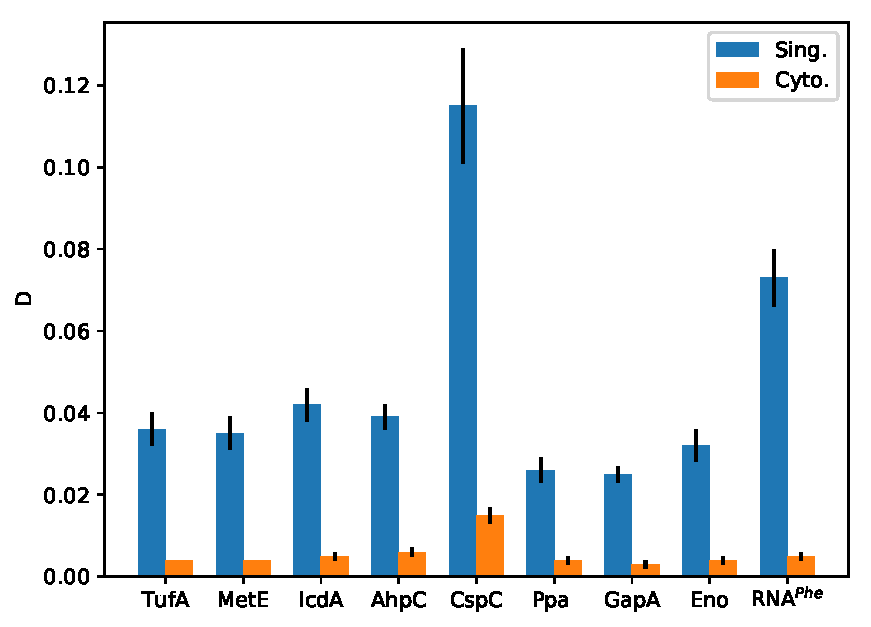
\includegraphics[scale=0.6]{msd.pdf}
\caption{Diffusion coefficient of crowders from single molecule simulations (blue bars) and cytoplasm simulations (orange bars).}
\end{figure}

\begin{figure}
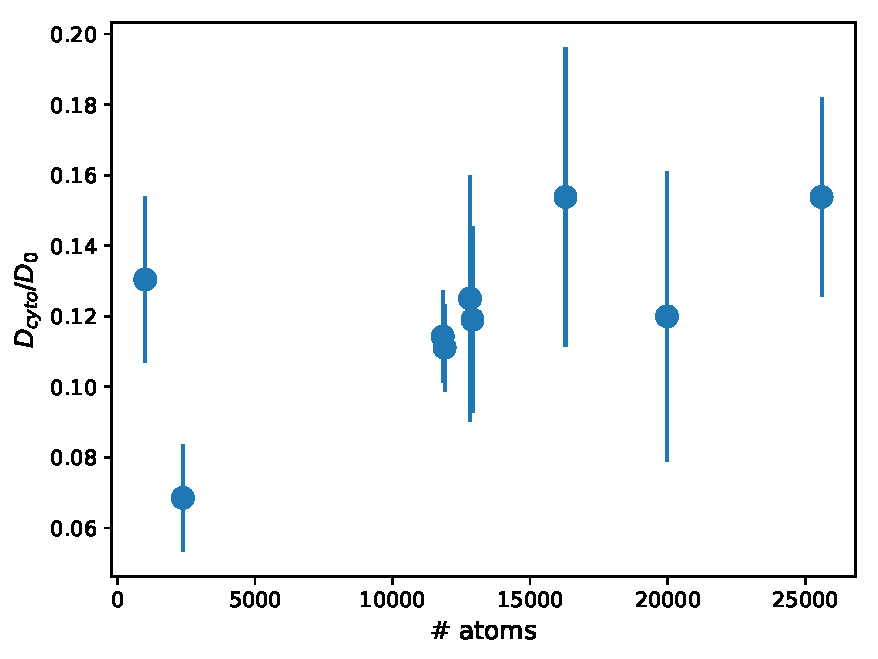
\includegraphics[scale=0.6]{diff_cyto_over_singles.pdf}
\caption{The ratio between diffusion coefficient obtained from cytoplasm to single molecule simulations. The crowders are sorted according to their sizes on the x-axis.}
\end{figure}



\subsubsection{Structural integrity of the crowders}
RMSD and SASA plots, show that the crowders didn't unfold


\begin{figure}
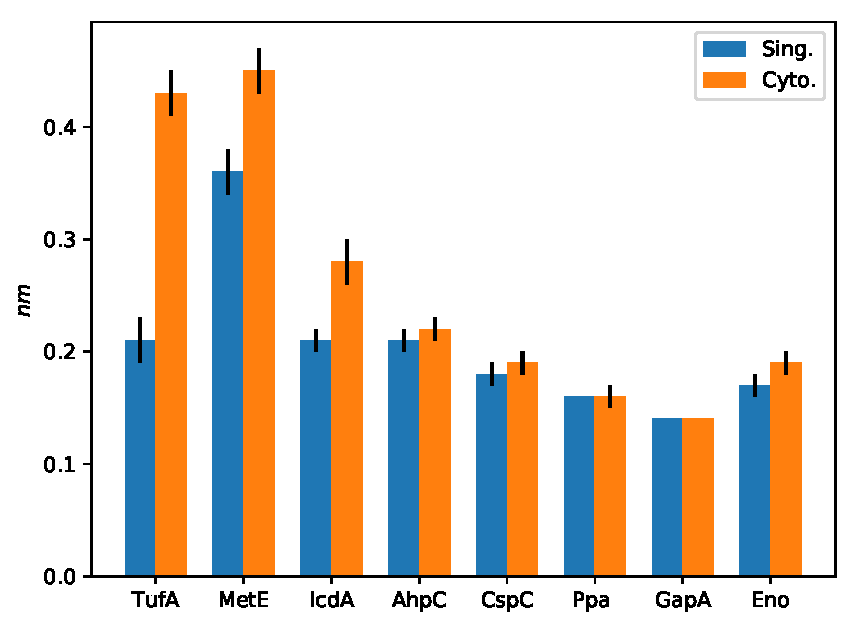
\includegraphics[scale=0.6]{rmsd.pdf}
\caption{Root mean squared displacement (rmsd) for 8 proteins from single molecule simulation (blue bars) and cytoplasm simulation (orange bars). The average rmsd for each protein in single molecule simulation is over number of chains of proteins and three replica. The average rmsd for each protein in cytoplasm simulation are over number of chains of proteins, number of appearance and three replica. The error bars show the standard errors.}
\end{figure}

\begin{figure}
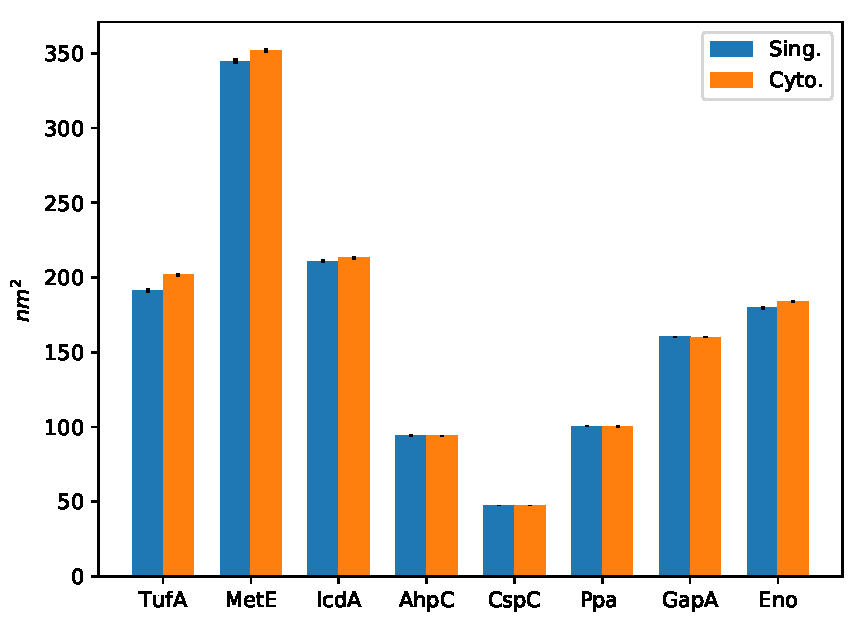
\includegraphics[scale=0.6]{sasa.pdf}
\caption{Solvent accessible surface area (sasa) for 8 proteins from single molecule simulation (blue bars) and cytoplasm simulation (orange bars). The average sasa for each protein in single molecule simulation is over number of chains of proteins and three replica. The average sasa for each protein in cytoplasm simulation are over number of chains of proteins, number of appearance and three replica. The error bars show the standard errors.}

\end{figure}

\subsubsection{Structural dynamics}
RMSF. Are there differences between the soup and single sim.?

\begin{figure}
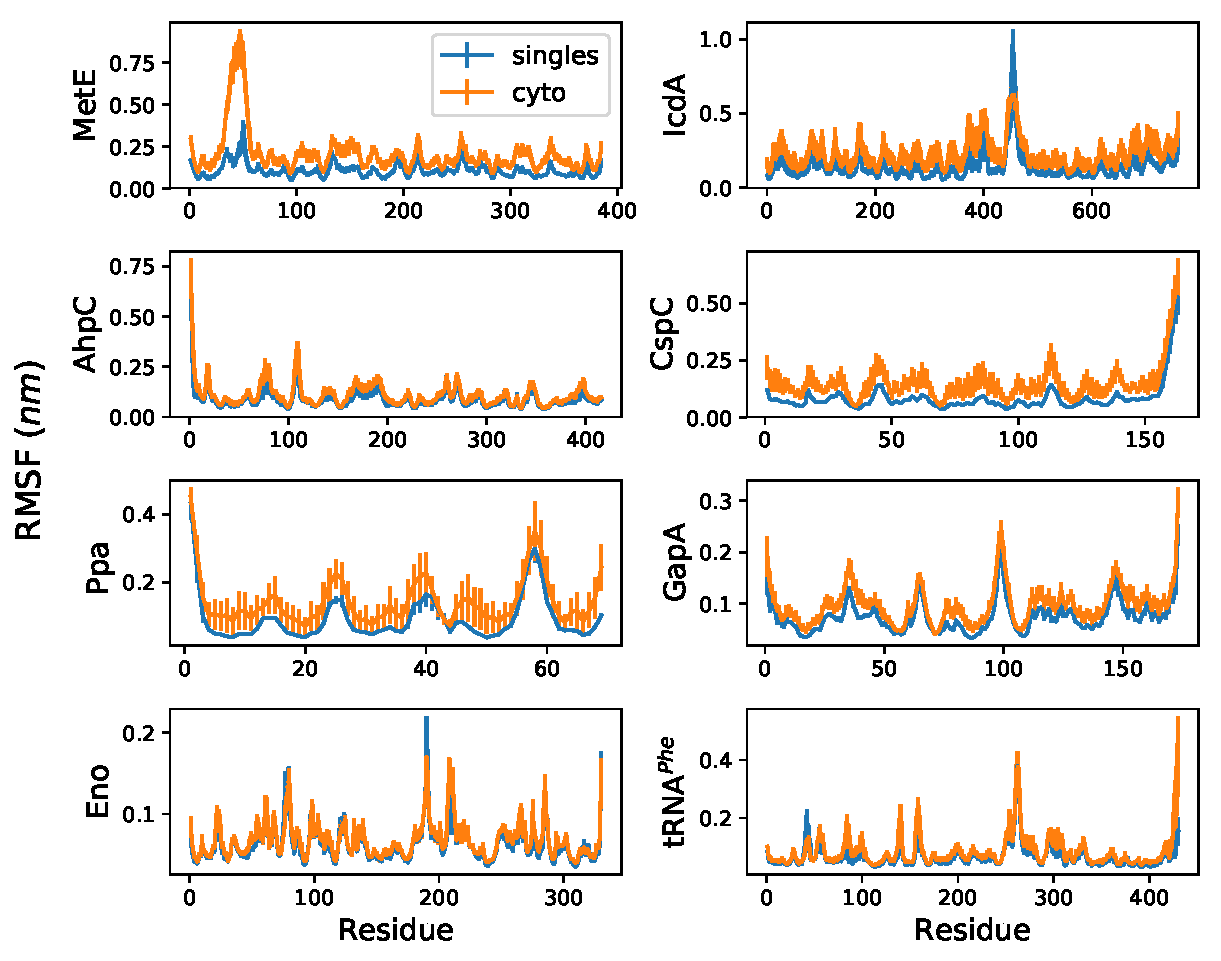
\includegraphics[scale=0.6]{rmsf.pdf}
\caption{Root mean squared fluctuations (rmsf) for 8 crowders from single molecule simulation (blue bars) and cytoplasm simulation (orange bars). x-axis shows the residues for each chain of proteins. The average rmsf for each protein in single molecule simulation is over number of chains of proteins and three replica. The average rmsd for each protein in cytoplasm simulation are over number of chains of proteins, number of appearance and three replica. The error bars show the standard errors.}
\end{figure}


\subsubsection{Oligomers under crowded condition}
\begin{figure}
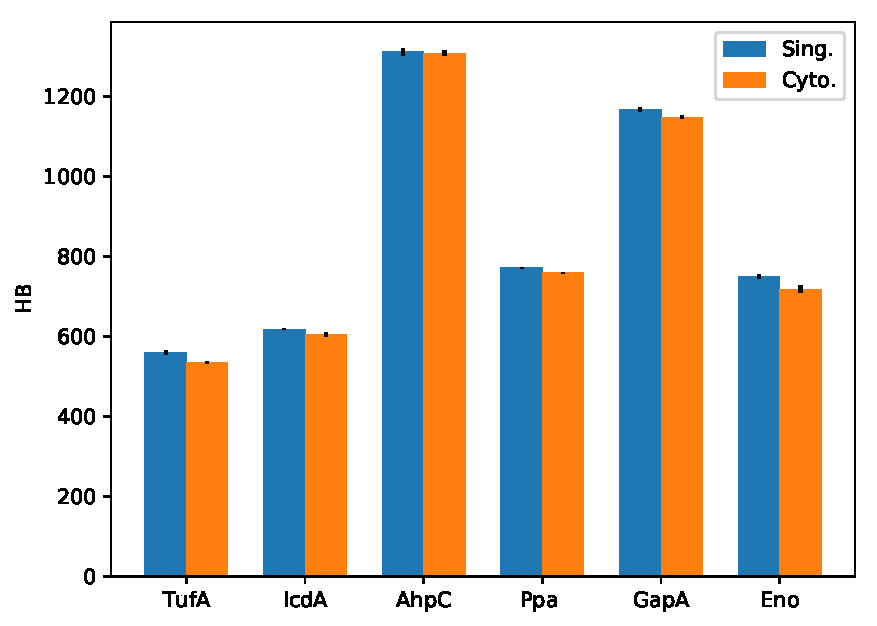
\includegraphics[scale=0.6]{hb.pdf}
\caption{Intramolecular hydrogen bonds (hb) for oligomers from single molecule simulation (blue bars) and cytoplasm simulation (orange bars). The average hydrogen bonds for each oligomer in single molecule simulation is over three replica. The average hydrogen bonds for each oligomer in cytoplasm simulation is over number of appearance of the oligomer in three replica. The error bars show the standard errors.}
\end{figure}


\subsubsection{Aggregation}
We observed aggregation of the metabolites that contain phosphate, ATP and FBP, with Mg2+ that was used as initially used as counter-ion for ATP and tRNA. After running simulations of small boxes containing just these metabolites and Mg2+, we found that completely protonating their phosphate groups can prevent aggregation. Thus, we advise caution when dealing with small molecules that are highly charged, such as ATP and FBP. Trial simulations with small boxes in which these metabolites are in high concentration to verify if they'll aggregate with Mg2+ or other charged species that are present in the box. In the specific case of ATP and FBP modeled with GAFF in boxes containing Mg2+, we advise that they should be completely protonated even though that is not their physiological protonation state. The topology and structure files we are providing for ATP and FBP on github are already protonated.

< FIGURE SHOWING THE AGGREGATION >
< FIGURE SHOWING THAT PROTONATED PHOSPHATE DOESN'T AGGREGATE >



\begin{figure}
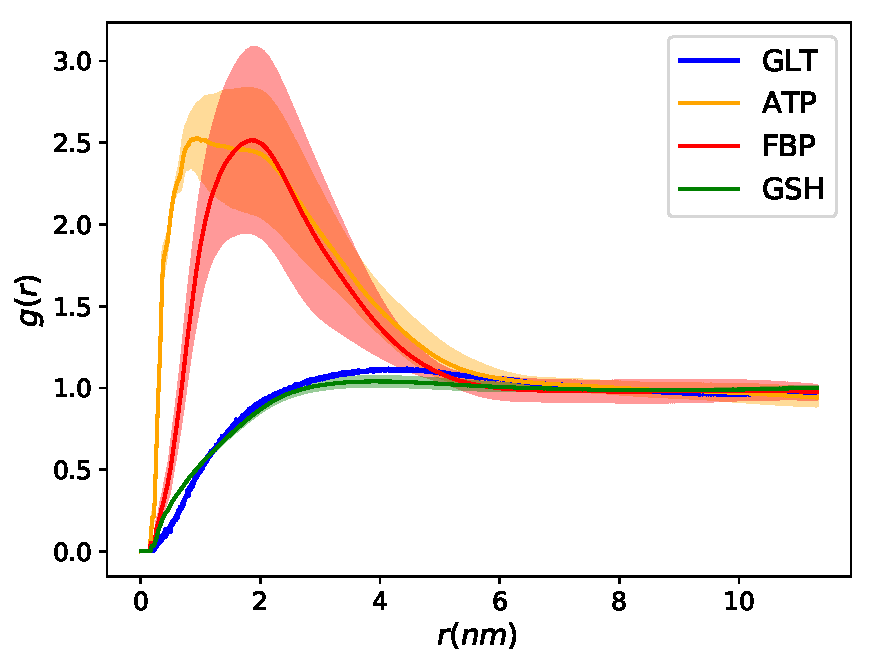
\includegraphics[scale=0.6]{rdf_RNA_metabolites.pdf}
\caption{Radial distribution function showing the probability of finding a metabolite around RNA molecules.}
\end{figure}

\begin{figure}
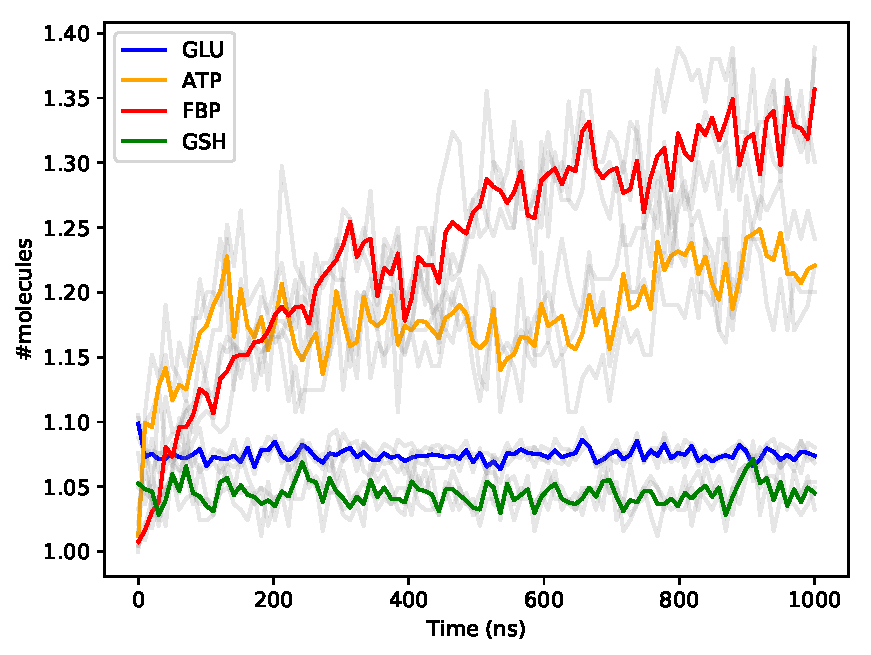
\includegraphics[scale=0.6]{avclust.pdf}
\caption{Number of metabolite molecules that form a cluster in cytoplasm simulations.}
\end{figure}

 
\section*{Discussion}\label{sec:dissc}
 

\bibliography{library}
% \begin{addendum}
%  \item  
%  \item[Competing Interests] 
%  \item[Correspondence]  
% \end{addendum}
 
\end{document}


